\documentclass{book}
\usepackage[utf8]{inputenc}
\usepackage[a4paper,total={6in,10in}]{geometry}

\usepackage{style}
\usepackage{thmtools}
\usepackage{thm-restate}

\usepackage{verbatim}
\usepackage[all,cmtip]{xy}

\usepackage{tikz-cd}
\newcommand{\cls}{\text{Class}}

%bib
\usepackage[square]{natbib}
\bibliographystyle{plainnat}


\title{Lecture Notes in Statistics}
\author{Kaizhao Liu}
\date{\today}

\begin{document}
\maketitle
\tableofcontents



\chapter{Introduction}
\section{In the Heartbeat of Our Real World}
Statistics is a discipline where we harness the power of numbers to understand data. Its relevance and applications are deeply intertwined with real-world scenarios. 
Therefore, a solid statistical analysis must first prove its merit in addressing real-world challenges before we delve into its mathematical underpinnings. 
This mirrors the approach in computational mathematics and probability theory.


However, this might appear starkly different from what you've heard about pure mathematics. 
Pure math often delves into areas like algebra, number theory, and combinatorics, or it might explore more philosophical realms like mathematical logic, or even bridge with theoretical physics through geometry and analysis. 
But at their core, these are all frameworks for modeling the world quantitatively. 
Take combinatorics, for instance: its essence would be lost if we were merely counting systems without origin or purpose. 
Similarly, what would be the point of studying geometry or topology if they didn't in some way reflect the world around us? 
A classic example is the advent of analysis. It began as a means to describe object motion but has since permeated countless fields. 
Even disciplines like number theory, which at first glance seem esoteric, have their roots in deeper philosophical pursuits, aiming for comprehensive understanding.

In essence, while pure mathematicians might appear to be delving into the profound, they're fundamentally exploring challenges that, albeit sometimes abstract, have ties to our tangible world. 
This interconnectedness between various fields and the real world underscores the essence of our research. 
After all, the real world remains the ultimate benchmark for the validity and relevance of our academic endeavors.


\section{The Enchanting Tapestry of Interdisciplinary Insights}
Statistics, inherently applied, finds its inspirations from the needs across diverse fields.  
This includes the sciences -- spanning computational science, physics, chemistry, biology, medicine, psychology, and geography -- as well as the liberal arts, encompassing economics, finance, sociology, semantics, aesthetics, and numerous others I haven't detailed here. 
Consequently, our research is deeply interdisciplinary. We value the influence of these diverse disciplines, incorporating their challenges and ideas, which enrich and elevate the realm of statistics. 
We keep with the pace of them.
Moreover, we recognize and harness profound mathematical advancements, arming ourselves with sophisticated tools and methods to address these multifaceted problems.

For instance, one of the early impacts of computer science on statistics was the development of bootstrap resampling. 
Prior to the computational revolution, statisticians heavily relied on stringent assumptions and theoretical derivations to make population inferences. 
These theoretical methods often imposed conditions that might not align with real-world data, such as assuming normal distributions or large sample sizes. 
However, with the advent of more powerful computers and advancements in computer science, Bradley Efron introduced the method of \textbf{bootstrap resampling} in the late 1970s. 
This innovative approach allows statisticians to resample or draw repeated samples from observed data, enabling the estimation of variability and confidence intervals for statistics without necessitating strict theoretical assumptions.

As another illustration, the influence of neuroscience on statistics is notably exemplified by the introduction of neural networks. 
Traditional statistical methods often make assumptions about data, such as linearity, independence, or homoscedasticity. 
While these methods have been robust and enduring, they can face challenges when confronted with complex, non-linear data structures prevalent in today's vast datasets. 
Neural networks, designed to mimic the intricate workings of the human brain's neurons, exhibit the capacity to model and capture intricate, non-linear relationships in data.


\section{Organization}
Let we restate, \textbf{the goal of statistics} is to deal with data encountered in our real world.
According to this goal, this lecture note focuses on the interplay between real world applications and theoretical development.
As this subject is applied in nature, many of our theoretical investigation are motivated by demand in various related areas,
such as sciences like computational science physics, chemistry, biology, psychology, or liberal arts like 




\chapter{Three Basic Objectives of Statistics}


\chapter{The Curse of Dimensionality}
Parallel to the development of the early twentieth century statistics, a new branch of science emerges, namely what we called computer science now.
They were first used for calculating bullets. The theory of computational mathematics also revives as this new computational tool appeared. 
Numerical methods for caculus, linear algebra, and differential equations are extensively studied and implemented in the computers.


\chapter{}

\chapter{Mathematical Statistics}

\section{Populations, Samples, and Models}
A typical statistical problem can be described ans follows:
\begin{enumerate}
\item (\textbf{planning experiments}) One or a series of random experiments is performed;
\item (\textbf{collecting data}) some data from the experiments are collected;
\item (\textbf{statistical analysis of the data}) extract information from the data, interpret the results, and draw some conclusions
\end{enumerate}
Statistical analysis of the data may contain:
\begin{itemize}
\item \textbf{descriptive data analysis}: such as the mean, median, range, standard deviation, etc., and some graphical displays, such as the histogram and box-and-whisker diagram, etc..
\item \textbf{statistical inference}
\item \textbf{decision theory}
\end{itemize}
We focus on more sophisticated methods of analyzing data, that is, the last two listed above.
\subsection{Populations and samples}
We formalize our statistics theory in the language of modern probability. First we need to specify some terms.
\begin{definition}[data set]
The data set is viewed as a \textbf{realization/observation} of a random element definitionined on a probability space ($\Omega,\mathcal{F},P$) related to the random experiment.
\end{definition}
\begin{definition}[population]
The probability measure $P$ is called the population.
\end{definition}
\begin{definition}[sample]
The random element that produces the data is called a \textbf{sample} from $P$. 
\end{definition}
\begin{definition}[known]
A population $P$ is known if and only if $P(A)$ is known for every event $A\in\mathcal{F}$.
\end{definition}
\subsection{Patametric and nonparametric models}
\begin{definition}[statistical model]
A statistical model is a set of assumptions on the population $P$ in a given problem. 
\end{definition}
\begin{remark}
It is often postulated to make the analysis possible or easy. Postulated models are often based on knowledge of the problem under consideration, and testing the correctness of them is also a task of statistical inference and decision theory.
\end{remark}
\begin{example}[parametric model]
The population $P$ is in a given parametric family $\mathcal{P}$.
\end{example}
\begin{example}[nonparametric model]
The population $P$ is in a given nonparametric family $\mathcal{P}$.
\end{example}
\begin{example}[semi-parametric model]
A nonparametric model having a parametric component.
\end{example}

\section{Statistics, Sufficiency, and Completeness}
\subsection{Statistics}
\begin{definition}[statistic]
A measurable function $T(X)$ of $X$ is called a statistic if $T$ is a known function.
\end{definition}
From a probabilistic point of view, the information within the statistic $T(X)$ is contained in the $\sigma-$field $\sigma(T(X))$. (This is because if two statistic generate the same $\sigma-$field, then there exist a bijection between them.) From this viewpoint, values of a statistic is non-material.\par
Any $T(X)$ is a random element. If the distribution of $X$ is unknown, then the distribution of $T(X)$ may also be unknown although $T$ is a known function. Finding the form of the distribution of $T(X)$ is one of the major problems in statistical inference and decision theory.
\subsection{Sufficiency and minimal sufficiency}
We now seek to describe a fully informative statistic $T(X)$. The concept definitionined below describes what we know by fully informative.
\begin{definition}[sufficiency]
Let $X$ be a sample from an unknown population $P\in\mathcal{P}$, where $\mathcal{P}$ is a family of populations. A statistics $T(X)$ is said to be sufficient for $P\in\mathcal{P}$ if and only if the conditional distribution of $X$ given $T$ is known (does not depend on $P$)
\end{definition}
\begin{remark}
The concept of syfficiency depends on the given family $\mathcal{P}$. If $T$ is sufficient for $P\in\mathcal{P}$, then $T$ is also sufficient for $P\in\mathcal{P}_0\subset\mathcal{P}$.
\end{remark}
This definitioninition can be interpreted as follows. Once we observe $X$ and compute a sufficient statistic $T(X)$, the original data $X$ do not contain any further information concerning the unknown population $P$ and can be discarded.\par
Finding a sufficient statistic in general involves a 'guess and verify' procedure. However, for families of populations having p.d.f's, a simple way of finding sufficient statistics is to use the factorization theorem.
\begin{theorem}[The factorization theorem]
Suppose that $X$ is a sample from $P\in\mathcal{P}$ and $\mathcal{P}$ is a family of probability measures on $(\mathbb{R}^n,\mathcal{B}^n)$ dominated by a $\sigma-$finite measure $\nu$. Then $T(X)$ is sufficient for $P\in\mathcal{P}$ if and only if there are nonnegative Borel functions $h$ (known) on $(\mathbb{R}^n,\mathcal{B}^n)$ and $g_P$ (unknown) on the range of $T$ such that
\[\frac{\mathrm{d} P}{\mathrm{d} \nu} =g_P(T(x))h(x)\]
\end{theorem}
For the proof of this theorem, we need a lemma concerning a family of probability measures.
\begin{lemma}
If a family $\mathcal{P}$ is dominated by a $\sigma-$finite measure, then $\mathcal{P}$ is dominated by a probability measure $Q=\sum_{i=1}^\infty c_iP_i$, where $c_i$'s are nonnegative constants with $\sum_{i=1}^\infty c_i=1$ and $P_i\in\mathcal{P}$.
\end{lemma}


Actually, there are many sufficient statistics for a given family $\mathcal{P}$, as the following theorem shows.
\begin{theorem}
If $T$ is a sufficient statistics and $T=\phi(S)$, where $\phi$ is measurable and $S$ is another statistics, then $S$ is sufficient.
\end{theorem}

\begin{remark}
Note that $\sigma(T)\subset\sigma(S)$ so $T$ provides a further reduction of the data than $S$.
\end{remark}
Therefore a question is raised. Is there a sufficient statistics that provides maximal reduction of the data?
\begin{definition}[minimal sufficiency]
Let $T$ be a sufficient statistic for $P\in\mathcal{P}$. $T$ is called a minimal sufficient statistic if and only if, for any other statistic $S$ sufficient for $P\in\mathcal{P}$, there is a measurable function $\phi$ such that $T=\phi(S)$ a.s. $\mathcal{P}$.
\end{definition}
\subsection{Completeness}
\begin{definition}[ancillary]
A statistic $V(X)$ is said to be ancillary if its distribution does not depend on the population $P$.
\end{definition}
\begin{definition}[first-order ancillary]
A statistic $V(X)$ is said to be first-order ancillary if $E[V(X)]$ is independent of $P$.
\end{definition}
Recalling the definitioninition of a complete orthogonal system in functional analysis, we definitionine the completeness of a statistic similarly. For a statistic $T(X)$, the measurable map $T:(\Omega,\mathcal{F})\longrightarrow(\mathcal{T},\mathcal{F}_\mathcal{T})$ induces a family of distributions $\mathcal{P}^T:=\left\{P\circ T^{-1}\right\}_{P\in\mathcal{P}}$ on $(\mathcal{T},\mathcal{F}_\mathcal{T})$. For $g:(\mathcal{T},\mathcal{F}_\mathcal{T})\longrightarrow(\mathbb{R},\mathcal{B})$ a $\mathcal{P}^T$ integrable Borel function, denote $\left\langle P,g\right\rangle_T:=E_P[g(T(X))]=\int_\mathcal{T}g\mathrm{d}P^T=P^T(g)$.
\begin{definition}[completeness]
A statistic $T(X)$ is said to be complete for $\mathcal{P}$ if and only if for any Borel function $g$ with $\left\langle P,g\right\rangle_T=0,\forall P\in\mathcal{P}$, we have $g=0$ a.s. $\mathcal{P}^T$.
\end{definition}
\begin{definition}[boundedly completeness]
A statistic $T(X)$ is said to be boundedly complete for $\mathcal{P}$ if and only if for any bounded Borel function $g$ with $\left\langle P,g\right\rangle_T=0,\forall P\in\mathcal{P}$, we have $g=0$ a.s. $\mathcal{P}^T$.
\end{definition}
\begin{remark}
If $T$ is (boundedly) complete and $S=\phi(T)$ for a measurable $\phi$, then $S$ is (boundedly) complete.
\end{remark}
\section{Statistical Decision Theory}
\subsection{Decision rules, loss functions, and risks}
Let $X$ be a sample from a population $P\in\mathcal{P}$. 
\begin{definition}[statistical decision]
A statistical decision is an \textbf{action} that one take after one observe $X$.
\end{definition}
\begin{definition}[action space]
Denote the set of allowable actions by $\mathbb{A}$. Let $\mathcal{F}_\mathbb{A}$ be a $\sigma$-field on $\mathbb{A}$. Then the measurable space $(\mathbb{A},\mathcal{F}_\mathbb{A})$ is called the action space.
\end{definition}
\begin{definition}[decision rule]
Let $\mathbf{X}$ be the range of $X$ and $\mathcal{F}_\mathbf{X}$ be a $\sigma$-field on $\mathbf{X}$. A decision rule is a known measurable function (a statistic) $T$ from $(\mathbf{X},\mathcal{F}_\mathbf{X})$ to $(\mathbb{A},\mathcal{F}_\mathbb{A})$.
\end{definition}
\begin{definition}[randomized decision rule]
A randomized decision rule is a function $\delta$ on $\mathbf{X}\times\mathcal{F}_\mathbb{A}$ s.t., for every $A\in\mathcal{F}_\mathbb{A}$ $\delta(\cdot,A)$ is a Borel function and, for every $x\in\mathbf{X}$ $\delta(x,\cdot)$ is a probability measure on $(\mathbb{A},\mathcal{F}_\mathbb{A})$.
\end{definition}
\begin{remark}
An alternate way to describe a randomized decision rule is to specify the method of \textbf{simulating} the action from $\mathbb{A}$ for each $x\in\mathbf{X}$.
\end{remark}
The construction or selection of decision rules cannot be done without any criterion about the performance of decision rules. In statistical decision theory, we set a criterion using a loss function.
\begin{definition}[loss function]
A loss function $L$ is a function from $\mathcal{P}\times\mathbb{A}$ to $[0,\infty)$ and is Borel on $(\mathbb{A},\mathcal{F}_\mathbb{A})$ for each fixed $P\in\mathcal{P}$.
\end{definition}
\begin{remark}
The loss function for a randomized rule $\delta$ is definitionined as \[L(P,\delta,x)=\int_\mathbb{A}L(P,a)\mathrm{d}\delta(x,a)\]
\end{remark}
A decision rule with small loss is preferred, but it is difficult to compare loss functions since they are random. For this reason, we introduce the risk function.
\begin{definition}[risk]
The risk of a decision rule $T$, which is the average loss for $T$, is definitionined to be \[ R_T(P)=E[L(P,T(X))]=\int_\mathbf{X}L(P,T(x))\mathrm{d}P_X(x)\]
\end{definition}
\begin{remark}
The risk of a randomized rule $\delta$ is definitionined as \[R_\delta(P)=E[L(P,\delta,X)]=\int_\mathbf{X}\int_\mathbb{A}L(P,a)\mathrm{d}\delta(x,a)\mathrm{d}P_X(x)\]
\end{remark}
\begin{definition}[as good as]
A rule $T_1$ is as good as another rule $T_2$ if and only if \[R_{T_1}(P)\le R_{T_2}(P) \text{   } \forall P\in\mathcal{P}\]
\end{definition}
\begin{remark}
If the inequality is strict for at least one $P\in\mathcal{P}$, we say $T_1$ is \textbf{better} than $T_2$.
\end{remark}
\begin{definition}[equivalent]
Two decision rules $T_1$ and $T_2$ are equivalent if and only if \[R_{T_1}(P)= R_{T_2}(P) \text{   } \forall P\in\mathcal{P}\]
\end{definition}
\begin{definition}[$\mathfrak{F}$-optimal]
Let $\mathfrak{F}$ be a class of decision rules. If there is a decision rule $T_*$ that is as good as any other rule in $\mathfrak{F}$, then $T_*$ is said to be $\mathfrak{F}$-optimal.
\end{definition}
\subsection{Admissibility and optimality}
Consider a given decision problem with a given loss $L(P,a)$.
\begin{definition}[admissibility]
Let $\mathfrak{F}$ be a class of decision rules. A decision rule $T\in\mathfrak{F}$ is called $\mathfrak{F}$-admissible if and only if there does not exist any $S\in\mathfrak{F}$ that is better than $T$.
\end{definition}

In view of the fact that an optimal rule often does not exist, statisticians adopt the following two approaches to choose a decision rule.\par
The first approach is to definitionine a class $\mathfrak{F}$ of decision rules that have some desirable properties and then try to find the best rule in $\mathfrak{F}$.
\begin{definition}[bias]
In an estimation problem, the bias of an estimator $T(X)$ of a real-valued parameter $\vartheta$ of the unknown population is definitionined to be $b_T(P)=E[T(X)]-\vartheta$. An estimator $T(X)$ is said to be unbiased for $\vartheta$ if and only if $b_T(P)=0$ for any $P\in\mathcal{P}$.
\end{definition}
\begin{definition}[invariance]

\end{definition}
The second approach is to consider some characteristic $R_T$ of $R_T(P)$ for a given decision rule $T$, and then minimize $R_T$ over $T\in\mathfrak{F}$.
\section{Statistical Inference}
In statisitical inference, we make an inference about the unknown population based on the sample $X$ and \textbf{inference procedure}, without using any loss function, although any inference procedure can be cast in decision-theoretic terms as a decision rule.\par
There are three main types of inference procedures: 
\begin{itemize}
\item \textbf{point estimators}
\item \textbf{hypothesis tests}
\item \textbf{confidence sets}
\end{itemize}
We will discuss them in the following sections.


\section{Asymptotic Criteria and Inference}
\subsection{Consistency}
\begin{definition}[consistency of point estimators]
Let $X=(X_1,\cdots,X_n)$ be a sample from $P\in\mathcal{P}$ and $T_n(X)$ be a point estimator of $\phi$ for every $n$.\par
(i) $T_n(X)$ is called consistent for $\phi$ if and only if $T_n(X)\to_p\phi$ w.r.t any $P\in\mathcal{P}$.\par
(ii) Let $\left\{a_n\right\}$ be a sequence of positive constants diverging to $\infty$. $T_n(X)$ is called $a_n$-consistent for $\phi$ if and only if $a_n[T_n(X)-\phi]=O_p(1)$ w.r.t. any $P\in\mathcal{P}$.\par
(iii) $T_n(X)$ is called strongly consistent for $\phi$ if and only if $T_n(X)\to\phi$ a.s. w.r.t. any $P\in\mathcal{P}$.\par
(iv) $T_n(X)$ is called $L_r$-consistent for $\phi$ if and only if $T_n(X)\to_{L_r}\phi$ w.r.t any $P\in\mathcal{P}$ for some fixed $r>0$.
\end{definition}
\begin{remark}
Consistency is actually a concept relating to a sequence of estimators.
\end{remark}

\subsection{Asymptotic Bias, Variance, and MSE}
\begin{definition}[asymptotic expectation]
Let $\xi,\xi_1,\xi_2,\cdots$ be random variables and $\left\{a_n\right\}$ be a sequence of positive numbers satisfying $a_n\to\infty$ or $a_n\to a>0$. If $a_n\xi_n\to_d\xi$ and $E\left|\xi\right|<\infty$, then $\frac{E\xi}{a_n}$ is called an asymptotic expectation of $\xi_n$.
\end{definition}
\begin{lemma}

\end{lemma}
\begin{theorem}[uniqueness of asymptotic expectation]
Let $\left\{\xi_n\right\}$ be a sequence of random variables. Suppose that both $\frac{E\xi}{a_n}$ and $\frac{E\eta}{b_n}$ are asymptotic expectations of $\xi_n$. Then one of the following three must hold:\par
(a) $E\xi=E\eta=0$;\par
(b) $E\xi\ne0,E\eta=0$, and $\frac{b_n}{a_n}\to0$; or $E\xi=0,E\eta\ne0$, and $\frac{a_n}{b_n}\to0$;\par
(c) $E\xi\ne0,E\eta\ne0$, and $\frac{\frac{E\xi}{a_n}}{\frac{E\eta}{b_n}}\to 1$.
\end{theorem}
\begin{proof}
According to the definitioninition, $a_n\xi_n\to_d\xi$ and $b_n\xi_n\to_d\eta$.\par
(i) If both $\xi$ and $\eta$ has a nondegenerate c.d.f's, then the result \par
(ii) Suppose that $\xi$ has a nondegenerate c.d.f. but $\eta$ is a constant. If $\eta\ne0$, then by Slusky's theorem $\frac{a_n}{b_n}\to \frac{\xi}{\eta}$, which is impossible since $\xi$ has a nondegenerate c.d.f..\par
(iii) Suppose that both $\xi$ and $\eta$ are constants. If $\xi=\eta=0$, the result follows. If $\xi\ne0$ and $\eta=0$, then $\frac{b_n}{a_n}\to 0$. If $\xi\ne0$ and $\eta\ne0$, then $\frac{b_n}{a_n}\to  \frac{\xi}{\eta}$.
\end{proof}

\subsection{Asymptotic Inference}
Statistical inference based on asymptotic criteria and approximations is called asymptotic statistical inference. We now focus on asymptotic hypothesis tests and confidence sets.
\begin{definition}
Let $X=(X_1,\cdots,X_n)$ be a sample from $P\in\mathcal{P}$ and $T_n(X)$ be a test for $H_0:P\in\mathcal{P}_0$ versus $H_1:P\in\mathcal{P}_1$.\par
(i) If $\limsup_n \alpha_{T_n}(P)\le \alpha$ for any $P\in\mathcal{P}_0$, then $\alpha$ is an asymptotic significance level of $T_n$.\par
(ii) If $\lim_{n\to\infty} \sup_{P\in\mathcal{P}_0}\alpha_{T_n}(P)$ exists, then it is called the limiting size of $T_n$.\par

\end{definition}
\section{Unbisaed Estimation}

\section{Estimation in Parametric Models}


\section{Hypothesis tests}

\section{Confidence sets}



\chapter{Multivariate Data Analysis}
\section{The Multivariate Normal Distributions}
\subsection{Asymptotic Distributions of Sample Means and Covariance Matrices}


\subsection{The Noncentral \texorpdfstring{$\chi^2$}{} and \texorpdfstring{$F$}{} Distributions}
\begin{definition}[generalized hypergeometric functions]
The generalized hypergeometric function is
\[\sideset{_{p}}{_q}{\operatorname{F}} (a_1,\cdots a_p;b_1,\cdots,b_q;z)=\sum_{n=0}^\infty \frac{(a_1)_k\cdots (a_p)_k}{(b_1)_k\cdots (b_q)_k}\frac{z^k}{k!}\]
where $(a)_k=a(a+1)\cdots (a+k-1)$
\end{definition}

For our purpose we will make use of the results in the following two lemmas. The first gives a special integral for $_0F_1$.
\begin{lemma}
\[\frac{\Gamma(\frac{n}{2})}{\Gamma(\frac{1}{2})\Gamma(\frac{n-1}{2})}\int_0^\pi e^{z\cos \theta}\sin^{n-2}\theta\mathrm{d}\theta=\sideset{_0}{_1}{\operatorname{F}}(\frac{n}{2};\frac{z^2}{4})\]
\end{lemma}
The second lemma shows that $\sideset{_{p+1}}{_q}{\operatorname{F}}$ is essentially a Laplace transform of $\sideset{_p}{_q}{\operatorname{F}}$.
\begin{lemma}
\[\int_0^\infty e^{-zt}t^{a-1}\sideset{_p}{_q}{\operatorname{F}}(a_1,\cdots,a_p;b_1,\cdots,b_p;kt)\mathrm{d}t=\Gamma(a)z^{-a}\sideset{_{p+1}}{_q}{\operatorname{F}}(a_1,\cdots,a_p,a;b_1,\cdots,b_q;kz^{-1})\]
for $p<q,\Re(a)>0,\Re(z)>0$ or $p=q,\Re(a)>0,\Re(z)>\Re(k)$.
\end{lemma}

\begin{theorem}
If $X$ is $N_n(\mu,I_n)$ then the random variable $Z=X^TX$ has the density function
\[e^{-\frac{\delta}{2}}\sideset{_0}{_1}{\operatorname{F}}(\frac{n}{2};\frac{\delta z}{4})\frac{1}{2^{\frac{n}{2}}\Gamma(\frac{n}{2})}e^{-\frac{z}{2}}z^{\frac{n}{2}-1}\quad(z>0)\]
where $\delta=\mu^T\mu$. $Z$ is said to have the noncentral $\chi^2$ distribution with $n$ degrees of freedom and noncentrality parameter $\delta$, to be written as $\chi^2_n(\delta)$.
\end{theorem}
\begin{corollary}
If $Z$ is $\chi^2_n(\delta)$ then its density function can be expressed as 
\[\sum_{k=0}^\infty P(K=k)g_{n+2k}(z)\quad (z>0)\]
where $K$ is a Poisson random variable with mean $\frac{\delta}{2}$, and 
\[g_r(z)=\frac{1}{2^{\frac{r}{2}}\Gamma(\frac{r}{2})}e^{-\frac{z}{2}}z^{\frac{r}{2}-1}\]
 the density function of the $\chi^2_r$ distribution.
\end{corollary}
\begin{theorem}
    If $Z$ is $\chi^2_n(\delta)$ then its characteristic function is 
\[\varphi_z(t)=(1-2it)^{\frac{n}{2}}e^{\frac{it\delta}{1-2it}}\]
\end{theorem}
\begin{corollary}
    $E(Z)=n+\delta$ and $\text{Var}(Z)=2n+4\delta$
\end{corollary}
\begin{corollary}
    If $Z_1$ is $\chi^2_{n_1}(\delta_1)$, $Z_2$ is $\chi^2_{n_2}(\delta_2)$, and $Z_1$ and $Z_2$ are independent, then $Z_1+Z_2$ is $\chi^2_{n_1+n_2}(\delta_1+\delta_2)$.
\end{corollary}
We now turn to the noncentral $F$ distribution. Recall that the usual central $F$ distribution is obtained by taking the ratio of two independent $\chi^2$ variables divided by their degrees of freedom.
The noncentral $F$ distribution is obtained by allowing the numerator variable to be noncentral $\chi^2$.
\begin{theorem}
    If $Z_1$ is $\chi^2_{n_1}(\delta)$,$Z_2$ is $\chi^2_{n_2}$, and $Z_1$ and $Z_2$ are independent, then 
    \[F=\frac{Z_1/n_1}{Z_2/n_2}\]
    has the density function 
    \[e^{-\frac{\delta}{2}}\sideset{_1}{_1}{\operatorname{F}}(\frac{n_1+n_2}{2};\frac{n_1}{2};\frac{\frac{n_1}{2n_2}\delta z}{1+\frac{n_1}{n_2}z})\times\frac{\Gamma(\frac{n_1+n_2}{2})}{\Gamma(\frac{n_1}{2})\Gamma(\frac{n_2}{2})}\frac{z^{\frac{n_1}{2}-1}(\frac{n_1}{n_2})^\frac{n_1}{2}}{(1+\frac{n_1}{n_2}z)^{\frac{n_1+n_2}{2}}}\quad z>0\]
$F$ is said to have the noncentral $F$ distribution with $n_1$ and $n_2$ degrees of freedom and noncentrality parameter $\delta$, to be written as $F_{n_1,n_2}(\delta)$.
\end{theorem}
\begin{corollary}
    $E(F)=\frac{n_2(n_1+\delta)}{n_1(n_2-2)}(n_2>2)$ and $\text{Var}(F)=2(\frac{n_2}{n_1})^2\frac{(n_1+\delta)^2+(n_1+2\delta)(n_2-2)}{(n_2-2)^2(n_2-4)}(n_2>4)$
\end{corollary}
\subsection{Quadratic Forms}
\begin{theorem}
If $X$ is $N_m(\mu,\Sigma)$, where $\Sigma$ is nonsingular, then \par
(i) $(X-\mu)^T\Sigma^{-1}(X-\mu)$ is $\chi^2_m$ \par 
(ii) $X^T\Sigma^{-1}X$ is $\chi^2_m(\delta)$ where $\delta=\mu^T\Sigma^{-1}\mu$
\end{theorem}

\begin{theorem}
    If $X$ is $N_m(\mu,I_m)$ and $B$ is an $m\times m$ symmetric matrix, then $X^TBX$ has an noncentral $\chi^2$ distribution if and only if $B$ is idempotent.
\end{theorem}

\subsection{Spherical and Elliptical Distributions}
\begin{definition}
    A $m\times 1$ random vector $X$ is said to have a spherical distribution if $X$ and $OX$ have the same distribution for all $O\in O(n)$.
\end{definition}

\begin{theorem}
    Let $X$ be $E_m(\mu,V)$, where $V$ is diagonal. If $X_1,\cdots,X_m$ are all independent then $X$ is normal.
\end{theorem}
\begin{proof}
    WLOG assume $\mu=0$. Then the characteristic function of $X$ has the form $\phi(t)=\psi(t^TVt)=\psi(\sum_{i=1}^m t_i^2v_{ii})$.
Since $X_1,\cdots,X_m$ are independent we have $ $
This equation is known as Hamel's euqation and its only continuous solution is $\psi(z)=e^{kz}$ for some constant $k$.
Hence the characteristic function of $X$ has the form $\phi(t)=e^{kt^TVt}$, and because it is a characteristic function, we must have $k\le 0$ which implies that $X$ has a normal distribution.
\end{proof}


\section{Multivariate Integration}
\subsection{Exterior Products}
For any matrix $X$, $\mathrm{d}(X)$ denotes the matrix of differentials $(\mathrm{d}x_{ij})$.\par 
For an arbitary $n\times m$ matrix $X$, the symbol $(\mathrm{d}X)$ will denote the exterior product of the $mn$ distinct elements of $\mathrm{d}X$:
\[(\mathrm{d}X):=\bigwedge _{j=1}^m \bigwedge _{i=1}^n \mathrm{d}x_{ij}\]\par 
For a symmetric $m\times m$ matrix $X$, the symbol $(\mathrm{d}X)$ will denote the exterior product of the $\frac{m(m+1)}{2}$ distinct elements of $\mathrm{d}X$:
\[(\mathrm{d}X):=\bigwedge _{1\le i\le j=1\le m} \mathrm{d}x_{ij}\]\par 


\subsection{The Multivariate Gamma Function}

\subsection{Miscellaneous Jacobians}

\subsection{Invariant Measures}

\chapter{von Mises Expansion}

\section{Int}

\begin{definition}[statistical functional]
    Let $X_1,\cdots,X_n$ be a sample from population with distribution function $F$ and let $T_n=T_n(X_1,\cdots,X_n)$ be a 
    statistic. If $T_n$ can be written as a functional $T$ of the empirical distribution $\hat{F}_n$, i.e. $T_n=T(\hat{F}_n)$ where $T$
    does not depend on $n$.
\end{definition}

\begin{example}
    Let $\phi$ be a real-valued function and let 
    \[ T_n=\frac{1}{n}\sum_{i=1}^{n}\phi(X_i).\] 
    Then for a general distribution $G$, the functional defined by 
    \[ T(G)=\int \phi(x) \mathrm{d}G(x) \] 
    satisfies $T_n(X_1,\cdots,X_n)=T(\hat{F}_n)$. Functional of this form is called linear statistical functional.
\end{example}

\begin{example}
    The sample $k$-th central moment $T_n=m_k=T_n(\hat{F}_n)$, where 
    \[ T(G)=\int [x-\int x\mathrm{d}G]^k \mathrm{d}G(x)\]
\end{example}

\section{Influence Function}
\begin{definition}[von Mises derivative]
    Let $X_1,\cdots,X_n$ be a sample and let $T$ be a functional on a convex set of d.f.'s containing all empirical d.f.'s and the population d.f. $F$.
    Let $G$ be a point in this convex set. Then the von Mises derivative $T'_F$ of $T$ at $F$ is defined by 
    \[ T'_F(G-F)=\frac{\mathrm{d}}{\mathrm{d}t} T(F+t(G-F))|_{t=0},\]
    if there exists a real-valued function $\phi_F(x)$ (independent of $G$) s.t. 
    \[ T'_F(G-F)=\int \phi_F(x)\mathrm{d}(G-F)(x).\] 
    We shall normalize $\phi_F(x)$ by making 
    \[\int \phi_F(x)\mathrm{d}F (x)=0 ,\]
    and call it the influence function.
\end{definition}





\section{Infinitesimal Jackknife}
Jackknife is a general tool for estimating the variance and reducing the bias.
The basic idea of Jackknife is to drop one observations and recompute the estimate using the remaining observations.
This is done for each observation, and the results are then combined to produce an estimate.


If we assign each observation a weight, then dropping one observation is identical to giving it weight of zero.
The Infinitesimal Jackknife




\section{Perturbing a Training Input}
How would the model's prediction change if a training input were modified?




\part{Causal Inference}

\chapter{Counterfactuals}


This chapter aims to present the basic idea of counterfactuals in the language of probability theory. 
In this way, I hope to introduce new concepts and structures to enrich probability theory, and borrow tools and insights from probability theory to study causal inference.
In the following I fix $(\Omega,\mathcal{F},\mathbb{P})$ to be a probability space.
\section{Binary Treatment}
 Let $X,Y$ be random variables on $\Omega$.
\begin{example}[binary treatment]\label{binary treatment}
    You can imagine $\Omega$ as the collection of all people being investigated, each element $\omega\in\Omega$ stands for a single person being investigated.
    Suppose $X$ is a binary treatment variable, where $X=1$ means 'treated' and $X=0$ means 'not treated'. Let $Y$ be some outcome varible such as the absence of disease.
    The goal is to study the relationship between $Y$ and $X$. 
\end{example}

\begin{definition}[potential decomposition]
    If a random variable $Y$ can be written as $Y=C_01_{A^c}+C_11_A$ where $C_0$ and $C_1$ are two random variables,
    then we say that $Y$ admits a potential decomposition $C_0,C_1$ w.r.t. $A$.
\end{definition}
\begin{remark}
    If $X=1_A$ is the binary treatment varible associated with $A$, then we also say that $Y$ admits a potential decomposition w.r.t $X$. 
    In this case, we can call $C_0,C_1$ the potential outcomes with the following interpretation: $C_0$ is the outcome if not 
    treated and $C_1$ is the outcome if treated.
\end{remark}

\begin{theorem}[existence]
    For any random variable $Y$ on $\Omega$ and any event $A\in\mathcal{F}$, there exists random variable $C_0$ and $C_1$ s.t. 
    \[Y=C_01_{A^c}+C_11_{A}.\]
\end{theorem}
This theorem is self-evident. We can look at the following cases, where we assume $X=1_A$ is a binary treatment variable. 
\begin{example}
    Let $C_0=C_1=Y$, then it is a potential decomposition of $Y$ w.r.t. $X$. In this example, the outcome is the same whether treated or not.
    We can interpret this as $X$ has no causal effect on $Y$.
\end{example}

\begin{example}
    Let $C_0=Y1_{D}$ and $C_1=Y1_E$, where $A^c\subset D$, $A\subset E$ and $D,E\in\mathcal{F}$, then it is a potential decomposition of $Y$ w.r.t. $X$. 
    In this example, $D,E$ can be chosen rather arbitarily. This shows that potential decomposition is not unique.
\end{example}
The problem of the above example is that we can decompose a random variable \textit{a posteriori}. 
To model the causal effect of the real world, we want the decomposition to be \textit{a priori}.
Namely, we are given a treatment $X$ and potential outcomes $C_0,C_1$ first, then we construct $Y$ naturally. 
We express this special type of potential decomposition more succinctly by
\begin{equation}
    Y=C_X,
\end{equation}
which is called the \textbf{consistency relationship}.


Now we can define statistics.

\begin{definition}[average causal effect]
    Define the average causal effect or average treatment effect to be
    \begin{equation}
        \theta=\mathbb{E}C_1-\mathbb{E}C_0.
    \end{equation}
\end{definition}

\section{}
\begin{definition}[counterfactual function]
    A random variable which is parameterized by $X$.
\end{definition}

\begin{definition}[causal regression function]
    Define the causal regression function to be 
    \begin{equation}
        \theta(x)=\mathbb{E}_\omega C(x,\omega).
    \end{equation}
    Note that $x$ is fixed.
\end{definition}



\chapter{CPDAG}

\section{PDAGs}

\begin{definition}[PDAG]
    An acyclic partially directed graph, or PDAG for short, is a graph that contains both directed and undirected edges. It is acyclic in the sense that it contains no directed cycles.
\end{definition}
\begin{remark}
    An acyclic directed graph, or DAG for short, can be regarded as a PDAG without undirected edges.
\end{remark}
Here we list some graph theoretical concepts for a PDAG.
\begin{itemize}
    \item The \textit{skeleton} of any PDAG is the undirected graph resulting from ignoring the directionality of every edge. 
    \item A \textit{v-structure} in a PDAG $\cG$ is an ordered triple of nodes $(x,y,z)$ such that $\cG$ contains the directed edges $x \rightarrow y$ and $z \rightarrow y$, and $x$ and $z$ are not adjacent in $\cG$.
    \item A \textit{clique} in a PDAG is a set of nodes for which every pair of nodes is adjacent.
\end{itemize}
We also list some notations for a PDAG.
\begin{itemize}
    \item We use $\Pi_x$ to denote the set of parents for node $x$ in a PDAG.
    \item We use $N_x$ to denote the set of neighbors of node $x$ in a PDAG.
    \item We use $N_{x,y} = N_x \cap N_y$ to denote the set of common neighbors of $x$ and $y$ in a PDAG.
    \item We use $\Omega_{x,y} = \Pi_x \cap N_y$ to denote the set of parents of node $x$ that are neighbors of node $y$ in a PDAG.
    %\item We say a directed edge $x \rightarrow y$ is \textit{covered} if $\Pi_x = \Pi_y \setminus x$. Similarly, we say an undirected edge is covered if $ \Pi_x = \Pi_y$.
\end{itemize}

\section{MECs}

Two network structures are equivalent if the set of distributions that can be represented using one of the structures is identical to the set of distributions that can be represented using the other.
\begin{theorem}\label{thm:verma}
    Two DAGs are Markov equivalent if and only if they have the same skeleton and the same v-structures.
\end{theorem}
\begin{proof}
    
\end{proof}


\begin{definition}[CPDAG]
    The CPDAG of a DAG $\cD$, denoted as $\cC$, is a PDAG that has the same skeleton as $\cD$, and an edge is directed in $\cC$ if and only if it has the same orientation in every equivalent DAG of $\cD$.
\end{definition}
We can distinguish two kinds of edges in a DAG according to its CPDAG. A directed edge of a DAG is \textit{compelled} if it occurs in the corresponding CPDAG, otherwise, the directed edge is \textit{reversible}, and the corresponding parents are reversible parents.

\section{A Transformational Characterization of MECs}
\begin{definition}
    A directed edge $x\rightarrow y$ is \textit{covered} if $\Pi_{y}=\Pi_{x}\cup\{x\}$.
\end{definition}

\begin{theorem}\label{thm:transformational}
    Let $\cG$ be any DAG containing the edge $x \rightarrow y$, and let $\cG'$ be the directed graph identical to $\cG$ except that the edge between $x$ and $y$ in $\cG'$ is oriented as $y\rightarrow x$. Then $\cG'$ is a DAG that is equivalent to $\cG$ if and only if $x\rightarrow y$ is a covered edge in $\cG$.
\end{theorem}


\section{Characterization of CPDAGs}
We introduce some terminologies and the main theorem.
\begin{itemize}
    \item A PDAG is called a \textit{chain graph} if it contains no semi-directed cycles.
    \item An undirected graph is \textit{chordal} if every cycle of length greater than or equal to 4 possesses a chord.
    \item A directed edge $v\rightarrow u$ in a PDAG $\cP$ is \textit{strongly protected} if $v\rightarrow u$ occurs in at least one of the four induced subgraphs of $\cP$ in Figure \ref{fig:stronglyprotected}.
\end{itemize}

\begin{figure}[h]
    \caption{Configurations where $v \rightarrow u$ is strongly protected.}
    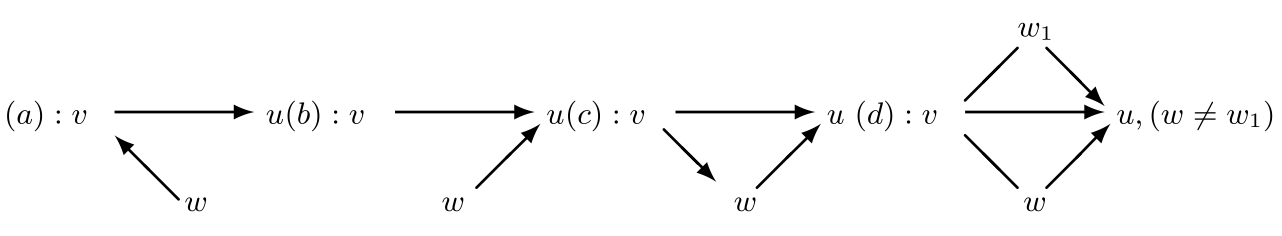
\includegraphics[width=\textwidth]{strongly protected.png}
    \label{fig:stronglyprotected}
\end{figure}


\begin{theorem}
    A graph $\cC$ is a CPDAG of a directed acyclic graph $\cD$ if and only if $\cC$ satisfies the following properties:
    \begin{enumerate}
        \item $\cC$ is a chain graph;
        \item let $\cC_\tau$ be the subgraph induced by $\tau$. $\cC_\tau$ is chordal for every chain component $\tau$;
        \item $w \rightarrow u - v$ does not occur as an induced subgraph of $\cC$;
        \item every arrow $v \rightarrow u$ in $\cC$ is strongly protected.
    \end{enumerate}
\end{theorem}
\begin{remark}
    
\end{remark}

The following series of lemma closely inspect a clique of size three in a CPDAG $\cC$, where there exists an undirected edge

\begin{lemma}\label{lem:0.4.1}
    The configuration $w \rightarrow u - v$ does not occur as an induced subgraph of $\cC$.
\end{lemma}
\begin{proof}
    If $w \rightarrow u - v$ occurs as an induced subgraph in $\cC$, then $w \rightarrow u \leftarrow v$ must occurs as a v-structure in some $\cD\sim\text{Class}(\cC)$. By Theorem \ref{thm:verma}, this is impossible.
\end{proof}



\begin{lemma}\label{lem:0.4.2}
    If 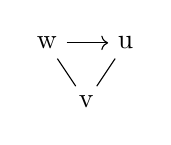
\begin{tikzpicture}[scale=0.5]
        % Nodes
        \node (w) at (0,0) {w};
        \node (u) at (2,0) {u};
        \node (v) at (1,-1.5) {v};
      
        % Edges
        \draw[->] (w) -- (u);
        \draw (v) -- (w);
        \draw (v) -- (u);
      \end{tikzpicture} 
      occurs in $\cC$, then there exist $\cD_1,\cD_2\in \text{Class}(\cC)$ such that 
      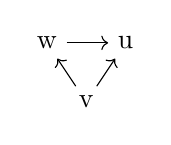
\begin{tikzpicture}[scale=0.5]
        % Nodes
        \node (w) at (0,0) {w};
        \node (u) at (2,0) {u};
        \node (v) at (1,-1.5) {v};
      
        % Edges
        \draw[->] (w) -- (u);
        \draw[->] (v) -- (w);
        \draw[->] (v) -- (u);
      \end{tikzpicture} occurs in $\cD_1$ and 
      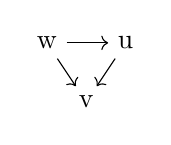
\begin{tikzpicture}[scale=0.5]
        % Nodes
        \node (w) at (0,0) {w};
        \node (u) at (2,0) {u};
        \node (v) at (1,-1.5) {v};
      
        % Edges
        \draw[->] (w) -- (u);
        \draw[->] (w) -- (v);
        \draw[->] (u) -- (v);
      \end{tikzpicture} occurs in $\cD_2$.
\end{lemma}
\begin{proof}
    Any $\cD\in\cls(\cC)$ must contain one of the followings:
    \[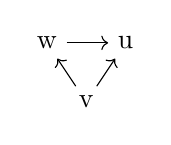
\begin{tikzpicture}[scale=0.5]
        % Nodes
        \node (w) at (0,0) {w};
        \node (u) at (2,0) {u};
        \node (v) at (1,-1.5) {v};
      
        % Edges
        \draw[->] (w) -- (u);
        \draw[->] (v) -- (w);
        \draw[->] (v) -- (u);
      \end{tikzpicture},\quad 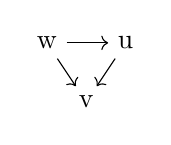
\begin{tikzpicture}[scale=0.5]
        % Nodes
        \node (w) at (0,0) {w};
        \node (u) at (2,0) {u};
        \node (v) at (1,-1.5) {v};
      
        % Edges
        \draw[->] (w) -- (u);
        \draw[->] (w) -- (v);
        \draw[->] (u) -- (v);
      \end{tikzpicture}, \quad 
      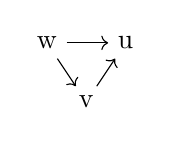
\begin{tikzpicture}[scale=0.5]
        % Nodes
        \node (w) at (0,0) {w};
        \node (u) at (2,0) {u};
        \node (v) at (1,-1.5) {v};
      
        % Edges
        \draw[->] (w) -- (u);
        \draw[->] (w) -- (v);
        \draw[->] (v) -- (u);
      \end{tikzpicture}.\]
    
\end{proof}

\begin{lemma}\label{lem:0.4.3}
    Let $\{w, u, v\}$ be any three nodes that form a clique of size three in $\cC$. If any two of the edges in the clique are undirected, then the third edge is undirected as well.
\end{lemma}
\begin{proof}
    Assume 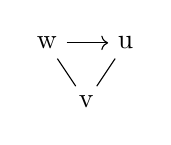
\begin{tikzpicture}[scale=0.5]
        % Nodes
        \node (w) at (0,0) {w};
        \node (u) at (2,0) {u};
        \node (v) at (1,-1.5) {v};
      
        % Edges
        \draw[->] (w) -- (u);
        \draw (v) -- (w);
        \draw (v) -- (u);
      \end{tikzpicture} occurs in $\cC$, we prove by contradiction. 
      According to Lemma \ref*{lem:0.4.2}, suppose 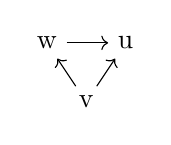
\begin{tikzpicture}[scale=0.5]
        % Nodes
        \node (w) at (0,0) {w};
        \node (u) at (2,0) {u};
        \node (v) at (1,-1.5) {v};
      
        % Edges
        \draw[->] (w) -- (u);
        \draw[->] (v) -- (w);
        \draw[->] (v) -- (u);
      \end{tikzpicture} occurs in $\cD_1$ and 
      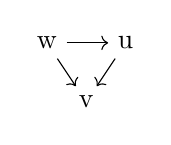
\begin{tikzpicture}[scale=0.5]
        % Nodes
        \node (w) at (0,0) {w};
        \node (u) at (2,0) {u};
        \node (v) at (1,-1.5) {v};
      
        % Edges
        \draw[->] (w) -- (u);
        \draw[->] (w) -- (v);
        \draw[->] (u) -- (v);
      \end{tikzpicture} occurs in $\cD_2$. \par
      As $w\rightarrow u$ is compelled, applying Theorem \ref{thm:transformational} to $\cD_1$ yields that $w\to u$ is not a covered edge in $\cD_1$.
      Therefore, there exists $x$ such that $x$ is a parent of $u$ but not a parent of $w$ in $\cG$. Now consider the subgraph induced by $\{u,v,w,x\}$ in $\cD_1$.
      If there is no edge between $x$ and $v$, then $x\rightarrow u \leftarrow v$ forms a v-structure, which is impossible. So there must be an edge between $x$ and $v$.\par 
      Now consider the subgraph induced by $\{u,v,w,x\}$ in $\cD_2$. As $x\rightarrow u \leftarrow w$ forms a v-structure in $\cD_1$, it also forms a v-structure in $\cD_2$ by Theorem \ref{thm:verma}. 
      Moreover, there must be an edge between $x$ and $v$. If $v\to x$, then $\cD_2$ contains a directed cycles. If $x\rightarrow v$ in $\cD_2$, then $x\rightarrow v \leftarrow w$ forms a v-structure, which is also impossible.

\end{proof}

\begin{lemma}\label{lem:0.4.4}
    Suppose there is a directed path from $v$ to $u$ in $\cC$. If there is an edge between $v$ and $u$, then it must be $v \rightarrow u$.
\end{lemma}
\begin{proof}
    Any $\cD\in\cls(\cC)$ must be acyclic.
\end{proof}

\begin{corollary}\label{cor:0.4.1.1}
    If $u - v$ is an undirected edge in $\cC$, then $\Pi_u = \Pi_v$.
\end{corollary}
\begin{proof}
    Suppose not. Without loss of generality, let $w$ be any parent of $u$ that is not a parent of $v$. 
    There are three configuration of the subgraph induced by $\{u,v,w\}$ in general: 
    \[\begin{tikzpicture}[scale=0.5]
        % Nodes
        \node (w) at (0,0) {w};
        \node (u) at (2,0) {u};
        \node (v) at (1,-1.5) {v};
      
        % Edges
        \draw[->] (w) -- (u);
        \draw (u) -- (v);
      \end{tikzpicture},\quad
    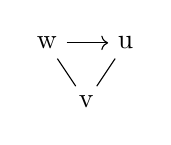
\begin{tikzpicture}[scale=0.5]
        % Nodes
        \node (w) at (0,0) {w};
        \node (u) at (2,0) {u};
        \node (v) at (1,-1.5) {v};
      
        % Edges
        \draw[->] (w) -- (u);
        \draw (w) -- (v);
        \draw (u) -- (v);
      \end{tikzpicture},\quad
      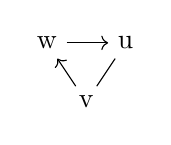
\begin{tikzpicture}[scale=0.5]
        % Nodes
        \node (w) at (0,0) {w};
        \node (u) at (2,0) {u};
        \node (v) at (1,-1.5) {v};
      
        % Edges
        \draw[->] (w) -- (u);
        \draw[->] (v) -- (w);
        \draw (u) -- (v);
      \end{tikzpicture}.\]
      The first case is excluded by Lemma \ref*{lem:0.4.1}, the second case is excluded by Lemma \ref*{lem:0.4.3}, and the third case is excluded by Lemma \ref*{lem:0.4.4}.
\end{proof}

Next we focus on the chain graph structure, \emph{i.e.} maximal undirected components in $\cC$.
A maximal undirected component $K$ of a CPDAG $\cC$ is a connected subgraph of $\cC$, where each connecting edge is undirected, and for every node $x \in K$, if there is an undirected edge $y-x$ in $\cC$, then $y\in K$.
For the remainder of this note, we use \textit{undirected component} to mean maximal undirected component.

\begin{lemma}\label{lem:0.4.6}
    For any directed edge $u \rightarrow v$ in $\cC$, $u$ is a parent of every node reachable by $v$ via undirected edges.
\end{lemma}
\begin{proof}
    Follows by a repeated application of Corollary \ref*{cor:0.4.1.1} along the edges in any undirected path.
\end{proof}

\begin{lemma}\label{lem:0.4.7}
    If there is a directed path of length one or more from $u$ to $v$ in $\cC$, then $u$ and $v$ are not in the same undirected component.
\end{lemma}
\begin{proof}
    Suppose not. Consider the last edge $w \rightarrow v$ in the directed path. By Lemma \ref*{lem:0.4.6}, $w$ is a parent of every node in the undirected component containing $v$, which means that $w$ is a parent of $u$. This forms a cycle.
\end{proof}

The next lemma shows that the undirected components of a CPDAG are chordal.
\begin{lemma}\label{lem:0.4.5}
    $\cC$ has no undirected chordless $k$-cycles $(k\geq 4)$.
\end{lemma}
\begin{proof}
    If an undirected chordless $k$-cycle occurs in $\cC$, then $\cC$ must have at least one v-structure in this cycle.
\end{proof}

\begin{corollary}
    Let $u$ and $v$ be any pair of nodes that are not adjacent in $\cC$. Then $N_{x,y}$ is a clique of undirected edges.
\end{corollary}

Now we consider the converse of Corollary \ref*{cor:0.4.1.1}.

\begin{lemma}
    If $v\rightarrow u$ is a directed edge in $\cC$, then $\Pi_u\neq \Pi_v\cup\{v\}$.
\end{lemma}
\begin{proof}
    
\end{proof}


\begin{lemma}
    Every directed edge $v\rightarrow u$ in $\cC$ is strongly protected.
\end{lemma}
\begin{proof}
    According to Lemma, we only need to show that if 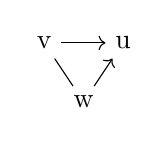
\begin{tikzpicture}[scale=0.5]
        % Nodes
        \node (w) at (0,0) {v};
        \node (u) at (2,0) {u};
        \node (v) at (1,-1.5) {w};
      
        % Edges
        \draw[->] (w) -- (u);
        \draw[->] (v) -- (u);
        \draw (v) -- (w);
      \end{tikzpicture} occurs in $\cC$, then the configuration (d) in Figure \ref{fig:stronglyprotected} occurs as an induced subgraph.
\end{proof}

Now we begin the proof of Theorem 
\begin{proof}
    We first prove the only if direction.
\end{proof}



\section{Algorithm: }


\section{Algorithm: }

\begin{definition}
    An operator is valid if
    \begin{itemize}
        \item the modified graph of the operator is a PDAG and has a consistent extension;
        \item 
    \end{itemize}
\end{definition}

\subsection{Compelled and Reversible Edge Insertions}
\begin{theorem}\label{thm:0.7.1}
    Let $\cC$ be any CPDAG for which nodes $x$ and $y$ are not adjacent. If the result of adding an edge between $x$ and $y$ is a PDAG that admits a consistent extension, then that edge is compelled if and only if $\Pi_x \neq \Pi_y$.
\end{theorem}
One reason that Theorem \ref*{thm:0.7.1} is difficult to prove is that after inserting edges into a CPDAG, edges that were reversible before can become compelled, and edges that were compelled before can become reversible.
In the following lemmas, we demonstrate a method for determining which edges in a CPDAG will necessarily remain compelled and reversible after an edge addition, based on the topology of the CPDAG.

\begin{lemma}
    Let $\cC$ be a CPDAG,and let $\cP$ denote the PDAG that results from an edge addition or deletion. If $\cP$ admits a consistent extension, then any compelled edge $x \rightarrow y$ in $\cC$ cannot be compelled in the opposite direction in $\cP$.
\end{lemma}
\begin{proof}
    
\end{proof}

\subsection{The InsertU Operator}
\begin{theorem}
    Let $x$ and $y$ be two nodes that are not adjacent in $\cC$. The insertion of the undirected edge $x - y$ is valid if and only if (1) every undirected path between $x$ and $y$ contains a node in $N_{x,y}$, and (2) $\Pi_x = \Pi_y$.
\end{theorem}

\subsection{The DeleteU Operator}
\begin{theorem}
    Let $x - y$ be an undirected edge in CPDAG $\cC$. The deletion of $x - y$ is valid if and only if $N_{x,y}$ is a clique of undirected edges.
\end{theorem}

\subsection{The InsertD Operator}
\begin{lemma}
    Let $\cC$ be a CPDAG that contains a semi-directed path from $x$ to $y$. If there exists a directed edge $z \rightarrow w$ in this path, then there exists a directed path from $z$ to $y$ in $\cC$.
\end{lemma}

\begin{theorem}
    Let $x$ and $y$ be any two nodes that are not adjacent in CPDAG $\cC$. The insertion of $x \rightarrow y$ is valid if and only if (1) every semi-directed path from $y$ to $x$ contains at least one node in $\Omega_{x,y}$, (2) $\Omega_{x,y}$ is a clique of undirected edges, and (3) $\Pi_x \ne \Pi_y$.
\end{theorem}

\subsection{The DeleteD Operator}
\begin{theorem}
    Let $x \rightarrow y$ be a directed edge in CPDAG $\cC$. The deletion of $x \rightarrow y$ is valid if and only if $N_y$ is a clique of undirected edges.
\end{theorem}

\subsection{The ReverseD Operator}
\begin{theorem}
    Let $x \rightarrow y$ be a directed edge in CPDAG $\cC$. The reversal of $x \rightarrow y$ is valid if and only if (1) every semi-directed path from $x$ to $y$ that does not include the edge $x \rightarrow y$ contains at least one node in $\Omega_{y,x} \cup N_y$, and (2) $\Omega_{y,x}$ is a clique of undirected edges.
\end{theorem}

\subsection{The MakeV Operator}
\begin{theorem}
    Let $x - z - y$ be any length-two undirected path in CPDAG $\cC$ such that x and y are not adjacent. Replacing the undirected edges with directed edges to create the v-structure $x \rightarrow z \leftarrow y$ is valid if and only if every undirected path between $x$ and $y$ contains a node in $N_{x,y}$.
\end{theorem}

\section{Algorithm: Reversible MCMC on MECs}

We need to show each operator has a reversible operator.

\subsection{The InsertU Operator}
\begin{theorem}
    Let $x$ and $y$ be two nodes that are not adjacent in $\cC$. The insertion of the undirected edge $x - y$ is reversible if and only if (1) every undirected path between $x$ and $y$ contains a node in $N_{x,y}$, and (2) $\Pi_x = \Pi_y$.
\end{theorem}

\subsection{The DeleteU Operator}
\begin{theorem}
    Let $x - y$ be an undirected edge in CPDAG $\cC$. The deletion of $x - y$ is valid if and only if $N_{x,y}$ is a clique of undirected edges.
\end{theorem}

\subsection{The InsertD Operator}
\begin{lemma}
    Let $\cC$ be a CPDAG that contains a semi-directed path from $x$ to $y$. If there exists a directed edge $z \rightarrow w$ in this path, then there exists a directed path from $z$ to $y$ in $\cC$.
\end{lemma}

\begin{theorem}
    Let $x$ and $y$ be any two nodes that are not adjacent in CPDAG $\cC$. The insertion of $x \rightarrow y$ is valid if and only if (1) every semi-directed path from $y$ to $x$ contains at least one node in $\Omega_{x,y}$, (2) $\Omega_{x,y}$ is a clique of undirected edges, and (3) $\Pi_x \ne \Pi_y$.
\end{theorem}

\subsection{The DeleteD Operator}
\begin{theorem}
    Let $x \rightarrow y$ be a directed edge in CPDAG $\cC$. The deletion of $x \rightarrow y$ is valid if and only if $N_y$ is a clique of undirected edges.
\end{theorem}


\subsection{The RemoveV Operator}
First we show that RemoveC is valid.
\begin{theorem}
    
\end{theorem}

Next we show that RemoveC is reversible.

\section{Counting Sizes of MECs}
\subsection{Size of MEC Determined by the Number of Vertices}
Let $\cU_{p,n}$ be an undirected and connected chordal graph (UCCG) with $p$ vertices and $n$ edges.




%\bibliography{bib}

\end{document}
